\documentclass[tikz,xcolor]{standalone}
%\usepackage[x11names]{xcolor}
\usepackage{tikz}
\usetikzlibrary{arrows.meta}%pag 16.2, cuando el crece el tamaño se cancela el hueco de uno de los modelos de flecha
\usetikzlibrary{decorations.pathreplacing}
\newcommand*{\tikzgrid}[2]{\draw[help lines](0,0)grid[step=0.2,lightgray,ultra thin](#1,#2);\draw[help lines](0,0)grid[gray](#1,#2);\foreach\x in{0,1,...,#1}\node[below]at(\x,0){\scriptsize\x};\foreach\y in{1,2,...,#2}\node[left]at(0,\y){\scriptsize\y};}

\begin{document}

%\tikz{\draw(0,0)rectangle(2mm,2mm);}%comando tikz para algo simple
% Se puede escoger otra opción.

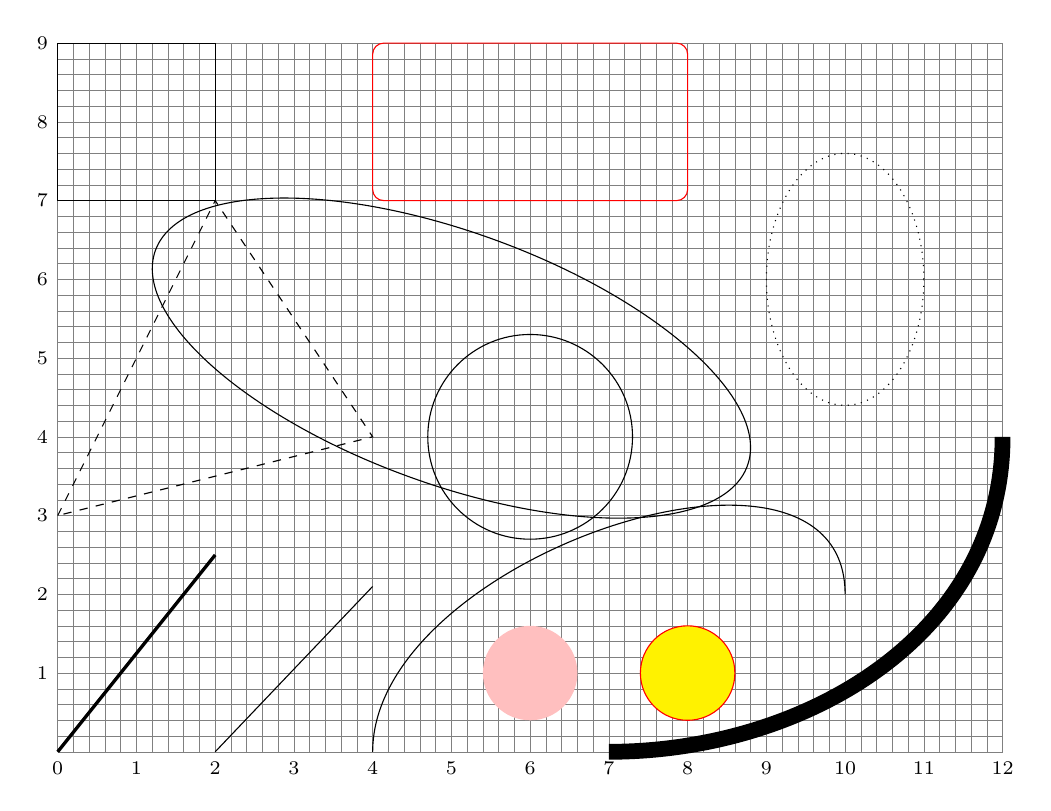
\begin{tikzpicture}
\tikzgrid{12}{9};% La unidad de longitud es 1cm , en picture también es de 1pt.
\path[draw,very thick](0,0)--(2,2.5);%Son equivalentes
\draw(2,0)--(4,2.1);
%\draw(0,3)--(2,7)--(4,4)--(0,3);%o es una figura cerrada, con punta.
\draw[dashed](0,3)--(2,7)--(4,4)--cycle;%figura cerrada.
\draw(0,7)|-(2,9);%hacia arriba y horizontal
\draw(0,7)-|(2,9);%horizontal y hacia arriba
\draw[rounded corners, red](4,7)rectangle(8,9);%puntas ovaladas o ¿biseladas?
\draw(6,4)circle[radius=1.3cm];
\draw[dotted](10,6)circle[x radius=1cm, y radius=1.6cm];
\draw(5,5)circle[x radius=4cm, y radius=1.6cm,rotate=160];%se rota en algo sexagesimal%uno es respecto al 0,0, el otro es rotar respecto al centro de la elipse
\draw[line width=2mm](7,0) to[out=0, in=270] (12,4);
\draw(4,0) to[out=90, in=90] (10,2);%control
\fill[pink](6,1)circle[radius=6mm];
\filldraw[color=yellow,draw=red](8,1)circle[radius=6mm];
%circulo y la circunferencia con el draw fill,con fill solo el interior
%\draw() to[out=]
\end{tikzpicture}
%!h es mas fuerte que h, pero no mas fuerte que H.
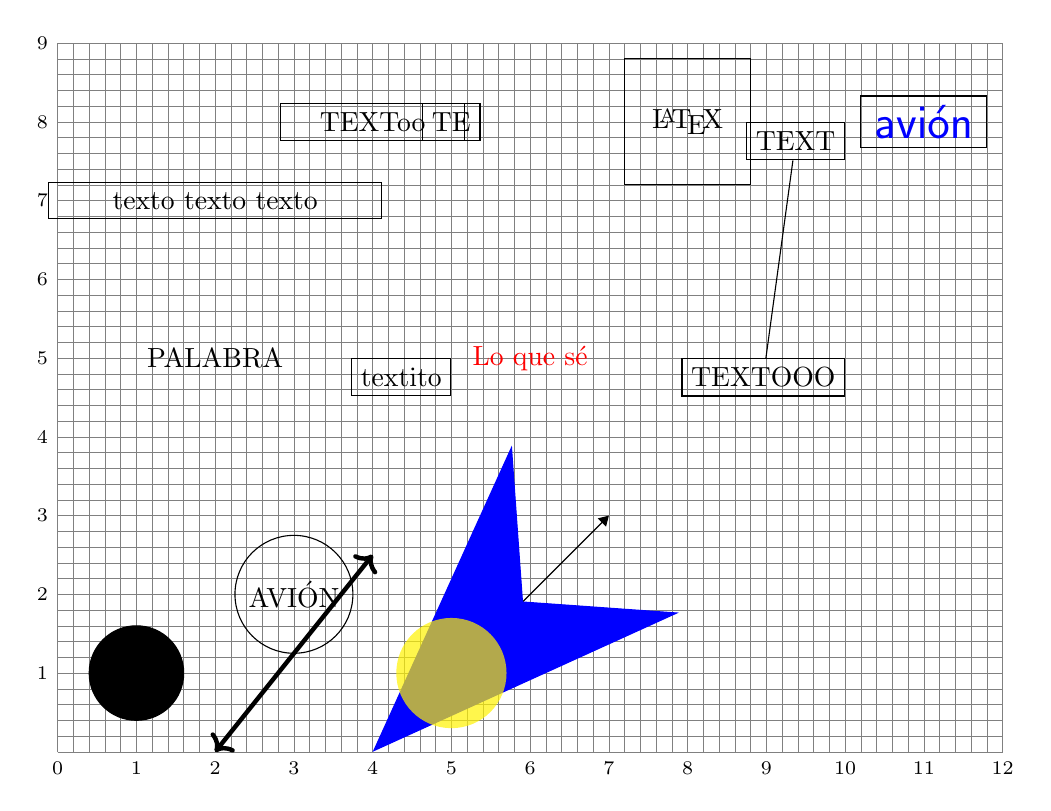
\begin{tikzpicture}
\tikzgrid{12}{9};
\useasboundingbox(0,0)rectangle(12,9);% Se puede usar en la carátula
\filldraw(1,1)circle[radius=6mm];
\draw[ultra thick,arrows=<->](2,0)--(4,2.5);%hasta la version 2, no se podia manipular las fechas, ni mover ni escalar, en la version 3.0 se mejoró con arrows
\draw[arrows={Stealth[scale=5,blue,length=8mm]}-Triangle](4,0)--(7,3);%es 40 mm, es 8 y se escala *5.
\fill[yellow,opacity=0.7](5,1)circle[radius=7mm];%existe el grado de opacidad, por defecto viene 1., 1 es opaco, 0 transparente
%lunes es la última clase, toploft 40 minutos, beamer 2 horas.
\node[red] at (6,5) {Lo que sé};
\node at (2,5) {PALABRA};%Hay dos formas de usar sin library
\node[draw,shape=circle] at (3,2) {AVIÓN};%existev la versión general
\node[draw,inner xsep=5mm]at(4,8){TEXToo};
\node[draw]at(5,8){TE};
\node[draw,minimum size=16mm] at(8,8) {\LaTeX};
\node[draw,minimum width=16mm,text=blue,font=\sffamily\LARGE]at(11,8){avión};
\node[draw,text width=4cm,align=center] at (2,7) {texto texto texto};%delimitando nodo
\node[draw,below left]at(5,5) {textito};%centrado es por defecto, con inner sep lo bajas a 0, tiene su punto de referencia.
%se puede unir las etiquestas
\node[draw, below left](AA)at(10,5){TEXTOOO};
\node[draw, below left](FF)at(10,8){TEXT};
\draw(AA)--(FF);
\end{tikzpicture}

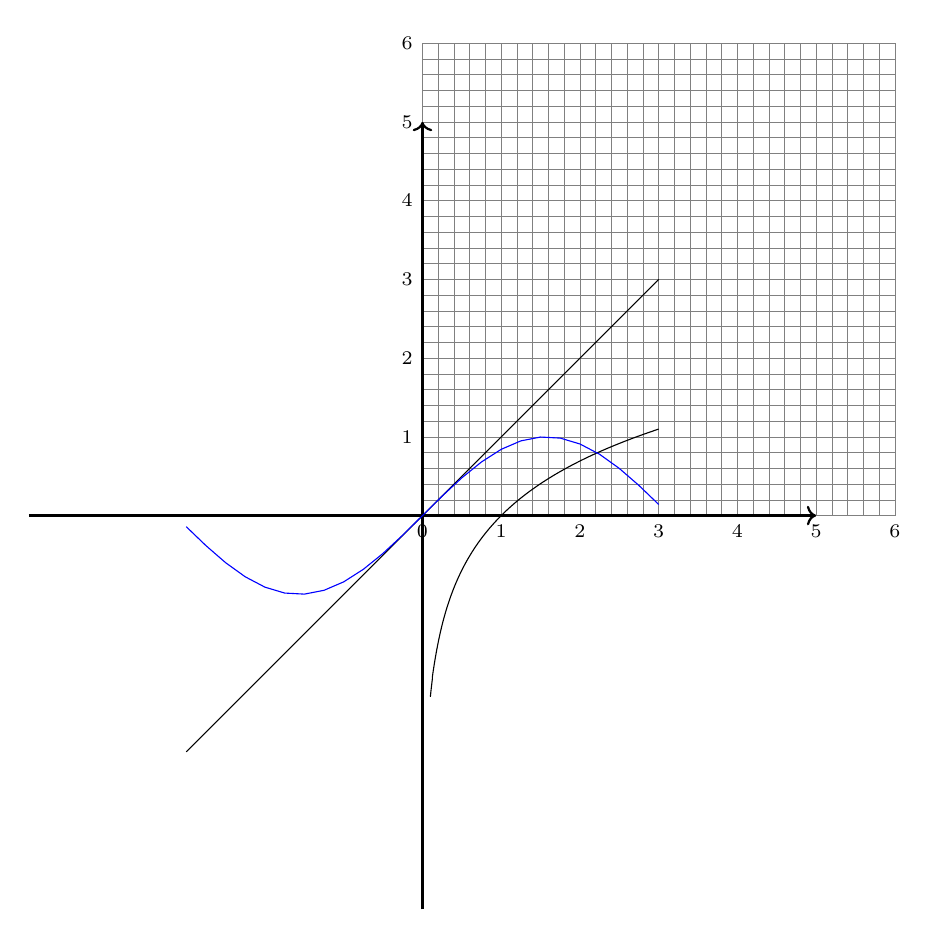
\begin{tikzpicture}
\tikzgrid{6}{6}
\draw[domain=-3:3] plot (\x,\x);
\draw[arrows=->,thick](-5,0) -- (5,0);
\draw[arrows=->,thick](0,-5) -- (0,5);
\draw[domain=0.1:3,samples=2000] plot(\x,{ln(\x)});%al terminar el nodo se muestra, ver manual pgf
\draw[blue,domain=-3:3] plot (\x,{sin(\x r)});
\end{tikzpicture}

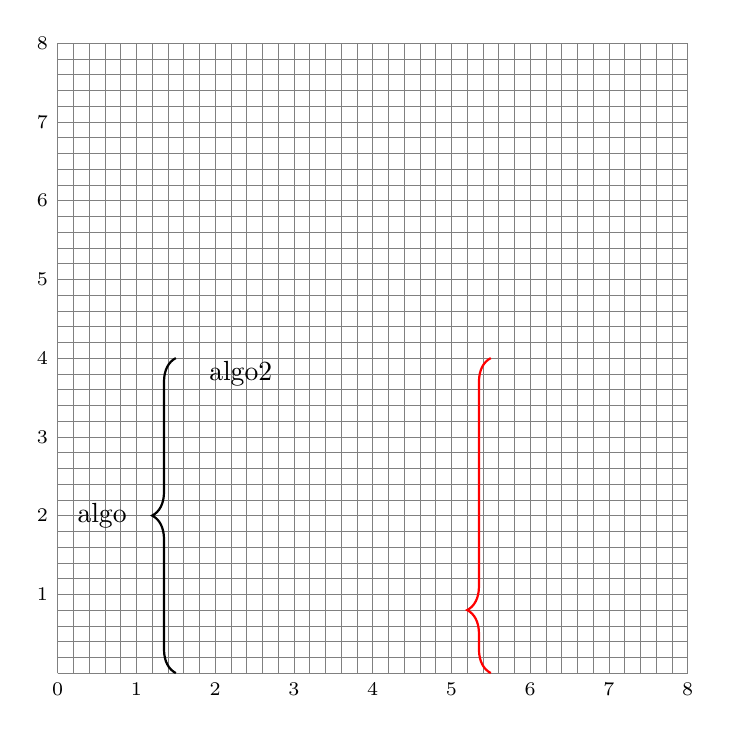
\begin{tikzpicture}%1ero con que va a decorar y luego que decorre
\tikzgrid{8}{8}
\draw[thick,decoration={brace,amplitude=3mm},decorate](1.5,0)--(1.5,4);
\node[left] at (1,2) {algo};
\node[right]at(1.8,3.8){algo2};
\draw[red,thick,decoration={brace,amplitude=3mm,aspect=0.2},decorate](5.5,0)--(5.5,4);
\end{tikzpicture}
\end{document}%version 3.0, 3.2, no es recomendable usar elipse
%la malla ayuda a dibujar

%diagrama o cuadro sinóptico.

%es un conjunto de macros dentro de tikz
es una manera amigable de usar pgf
tikz en si no es un paquete, pgf, tikz es pgf como latex es a tex.
Es sobre para hacer adornos.
Tiene como 10 años, es relativamente, hacer circunferencias, no era fácil.

tikz va después de color
Se necesita un eje de coordenadas.
% Pensando en las generaciones futuras.

existe un entorno scope dentro de tikzpciture para cosas locales.

el line width se define, los demás ya están definidos.


%se puede declarar con thickset.
% se recomienda ver thick o vertyhick
densamente, escasamente, dashed es guiones.

%encabezado de las secciones centrado, derecha, color.

8,12(4,8).